\newpage
\pagestyle{empty}    % 清空页码                                      %
\begin{figure}[h!]
\centering
\vspace{+0.2in}
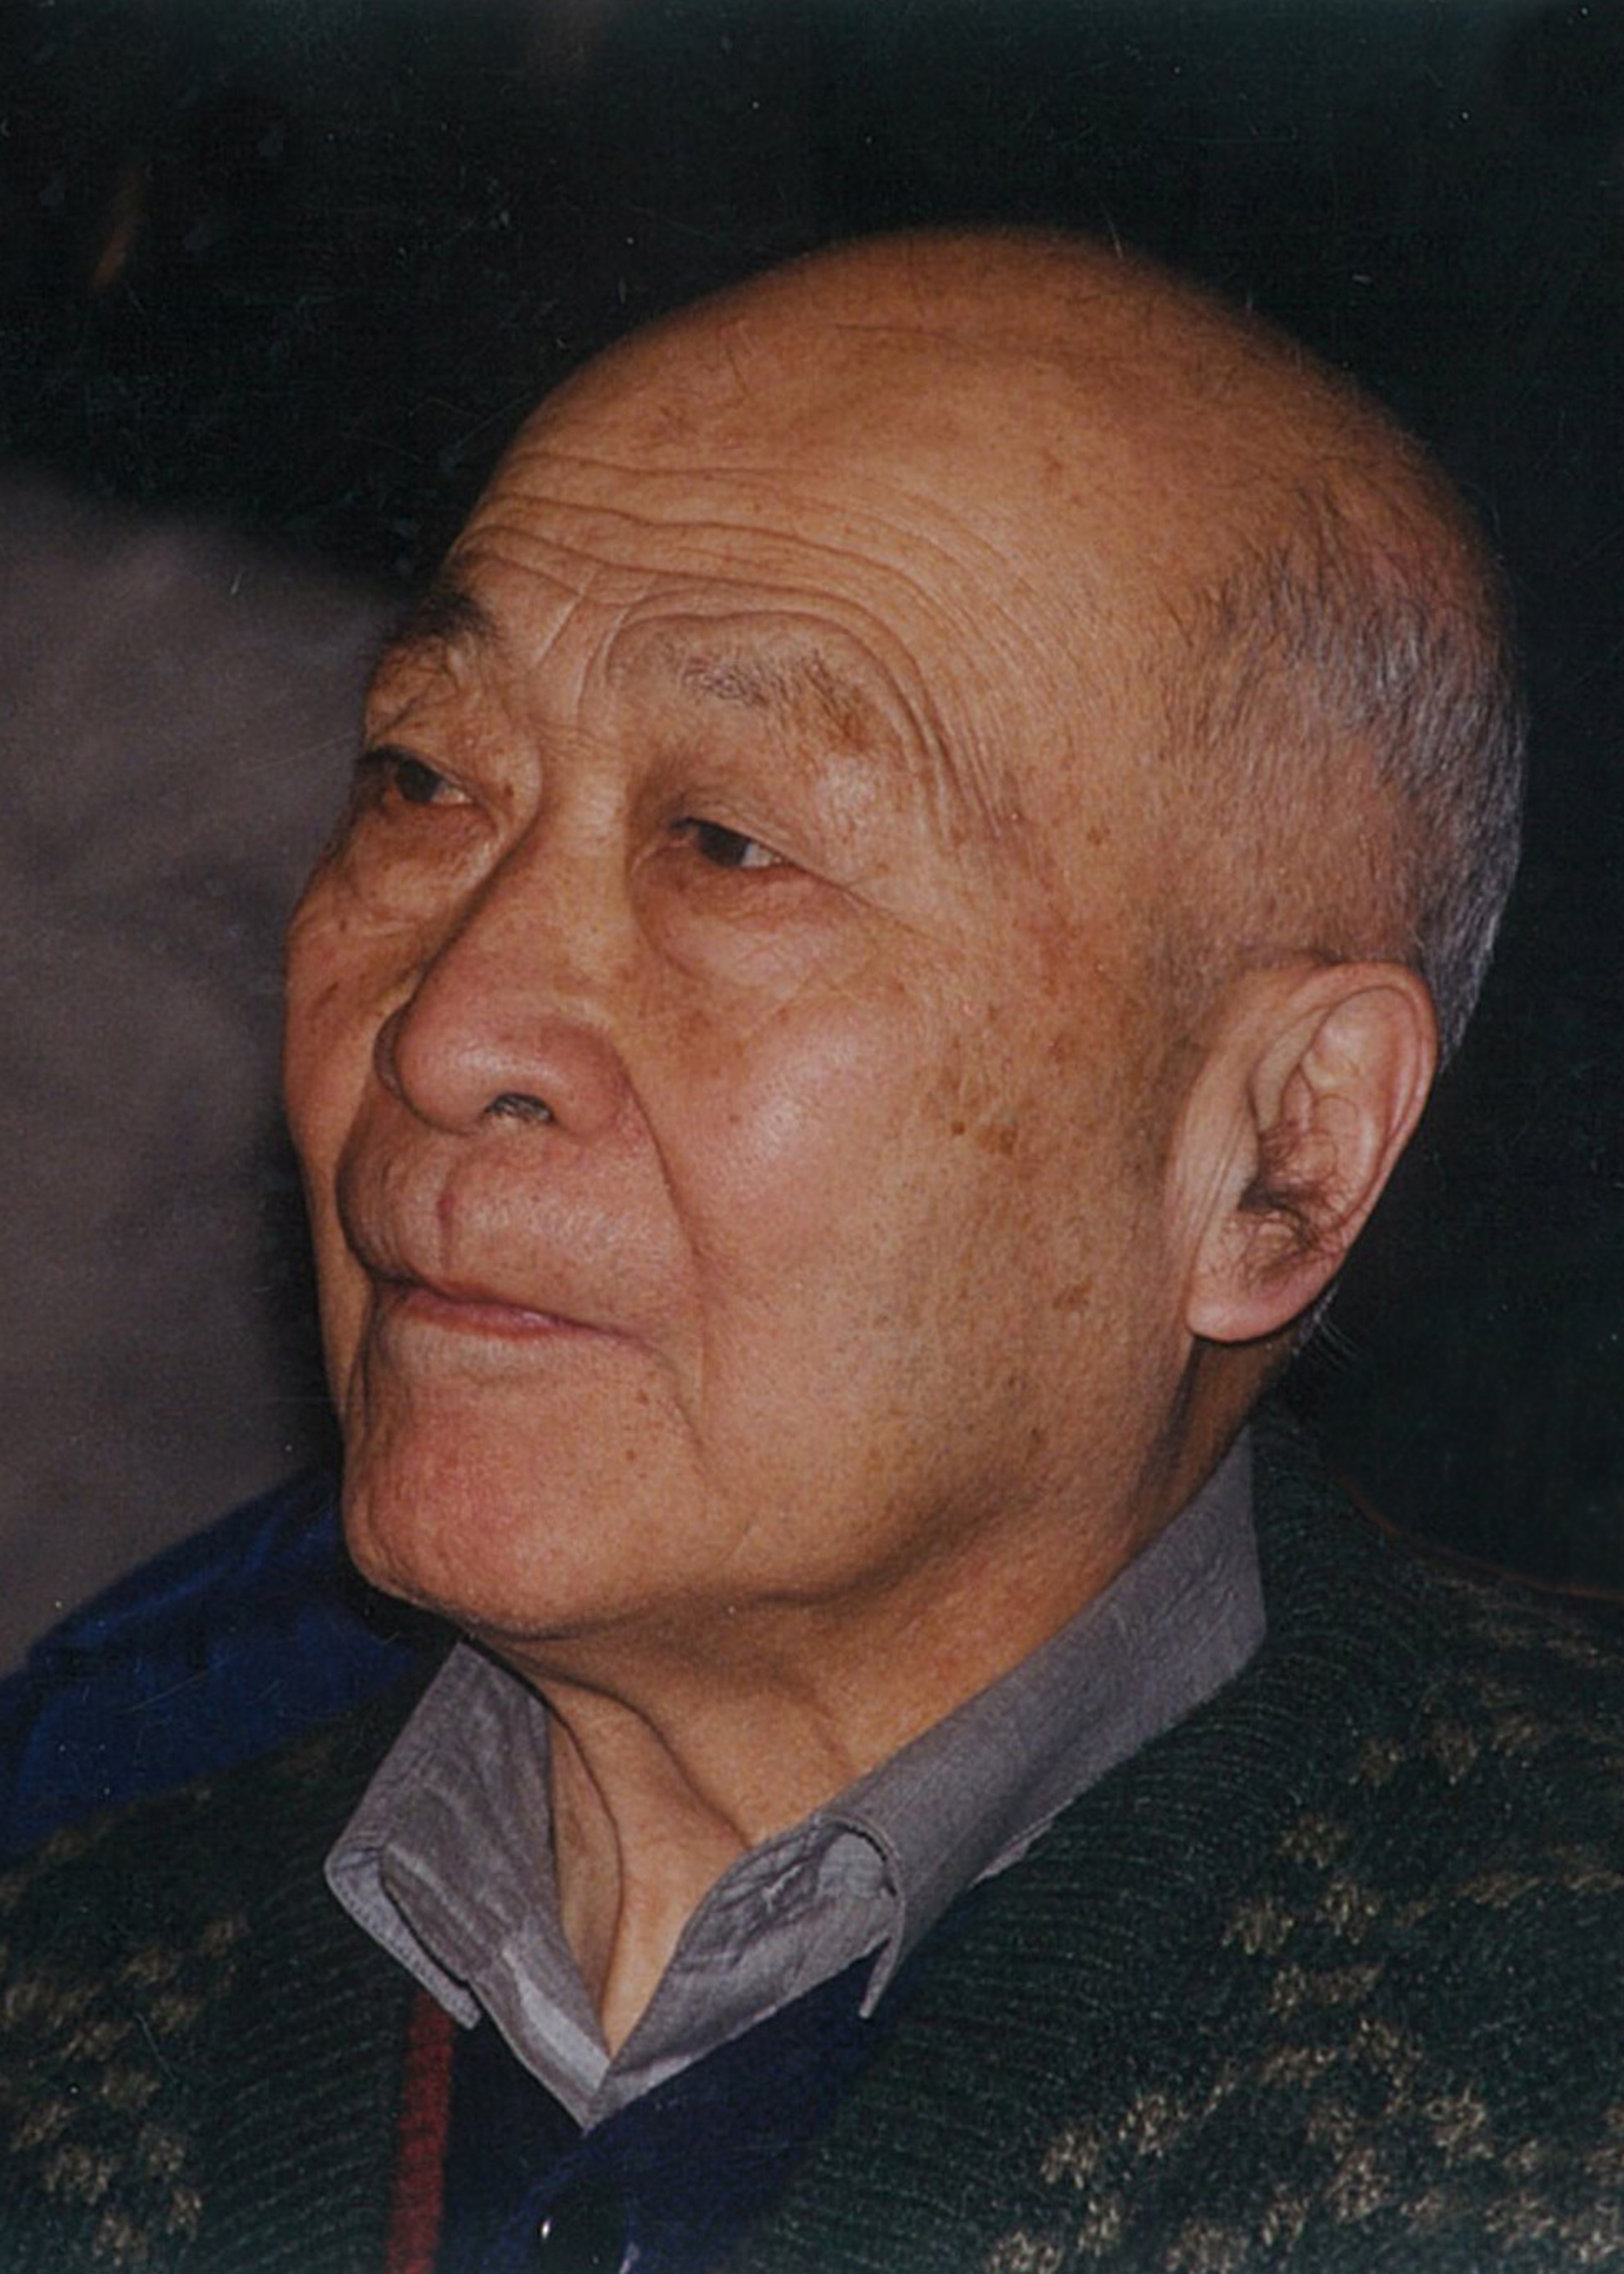
\includegraphics[height=1.20\textwidth,width=0.82\textwidth,viewport=0 0 360 520,clip]{Liu_Zengfu.jpg}
\caption*{\hei 刘曾复~教授~~(1914.11.9-2012.6.27)}
\label{Liu_Zengfu}
\end{figure}

\newpage
\begin{figure}[h!]
\centering
%\vspace{+0.2in}
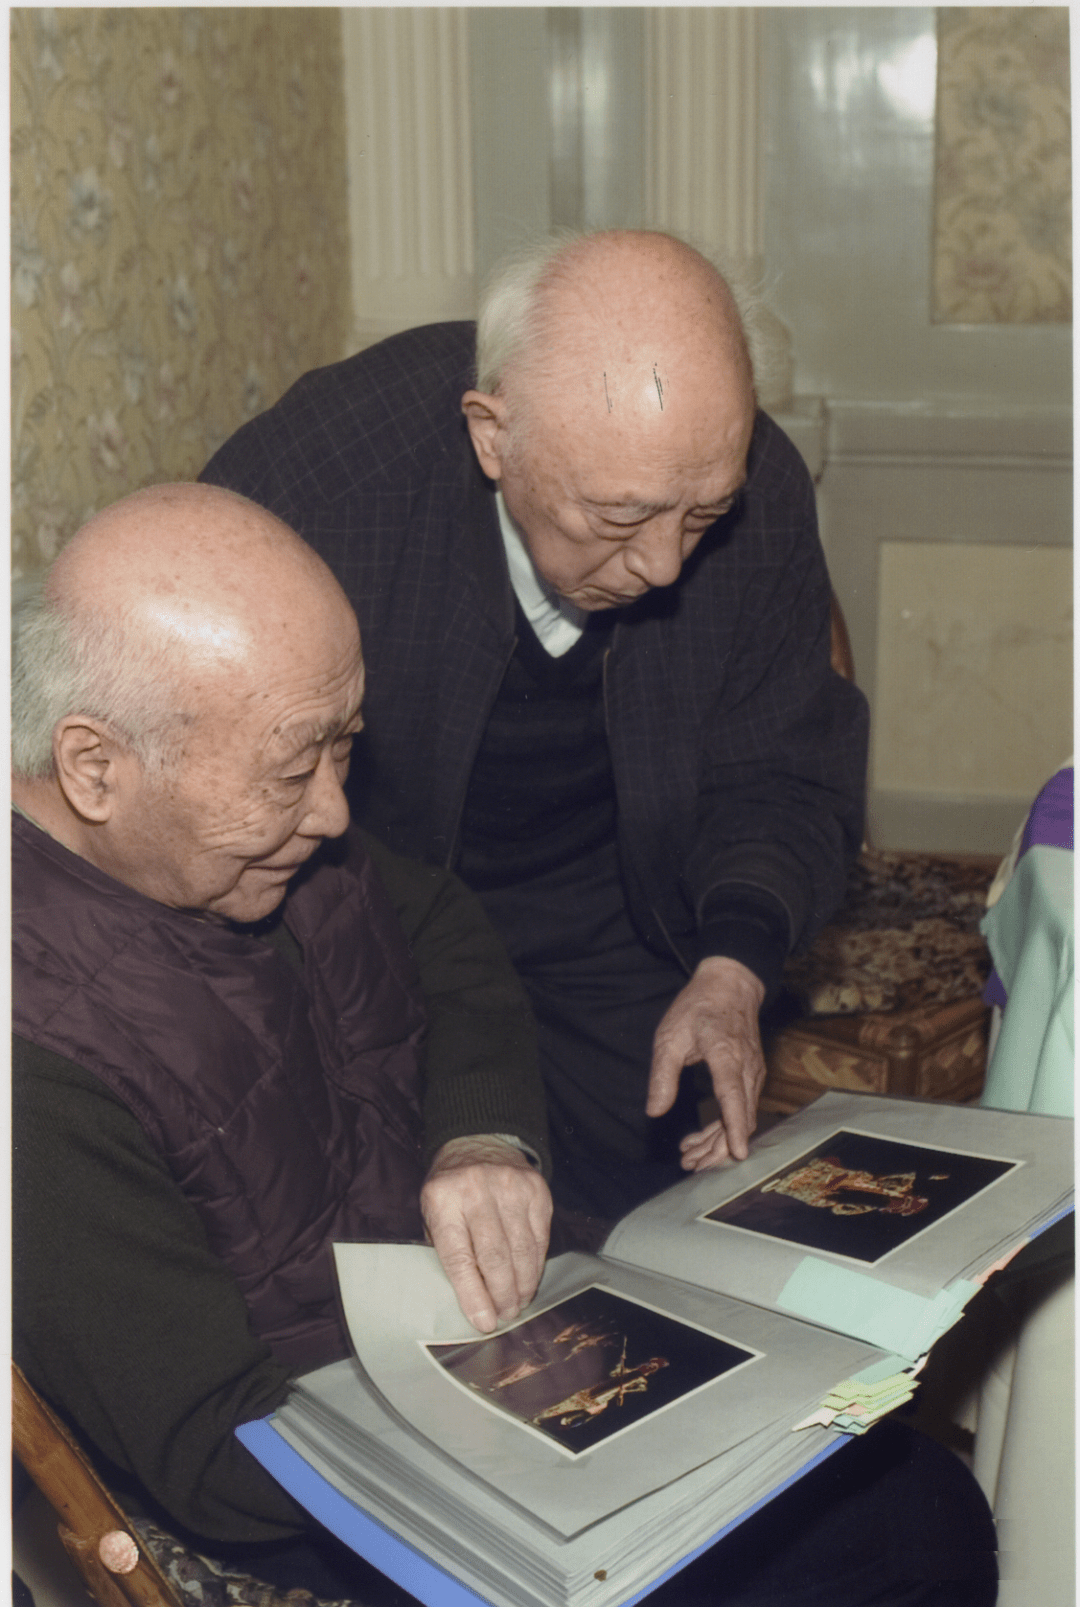
\includegraphics[height=1.38\textwidth,width=1.0\textwidth,viewport=0 0 1050 1550,clip]{Liu-Wu.png}
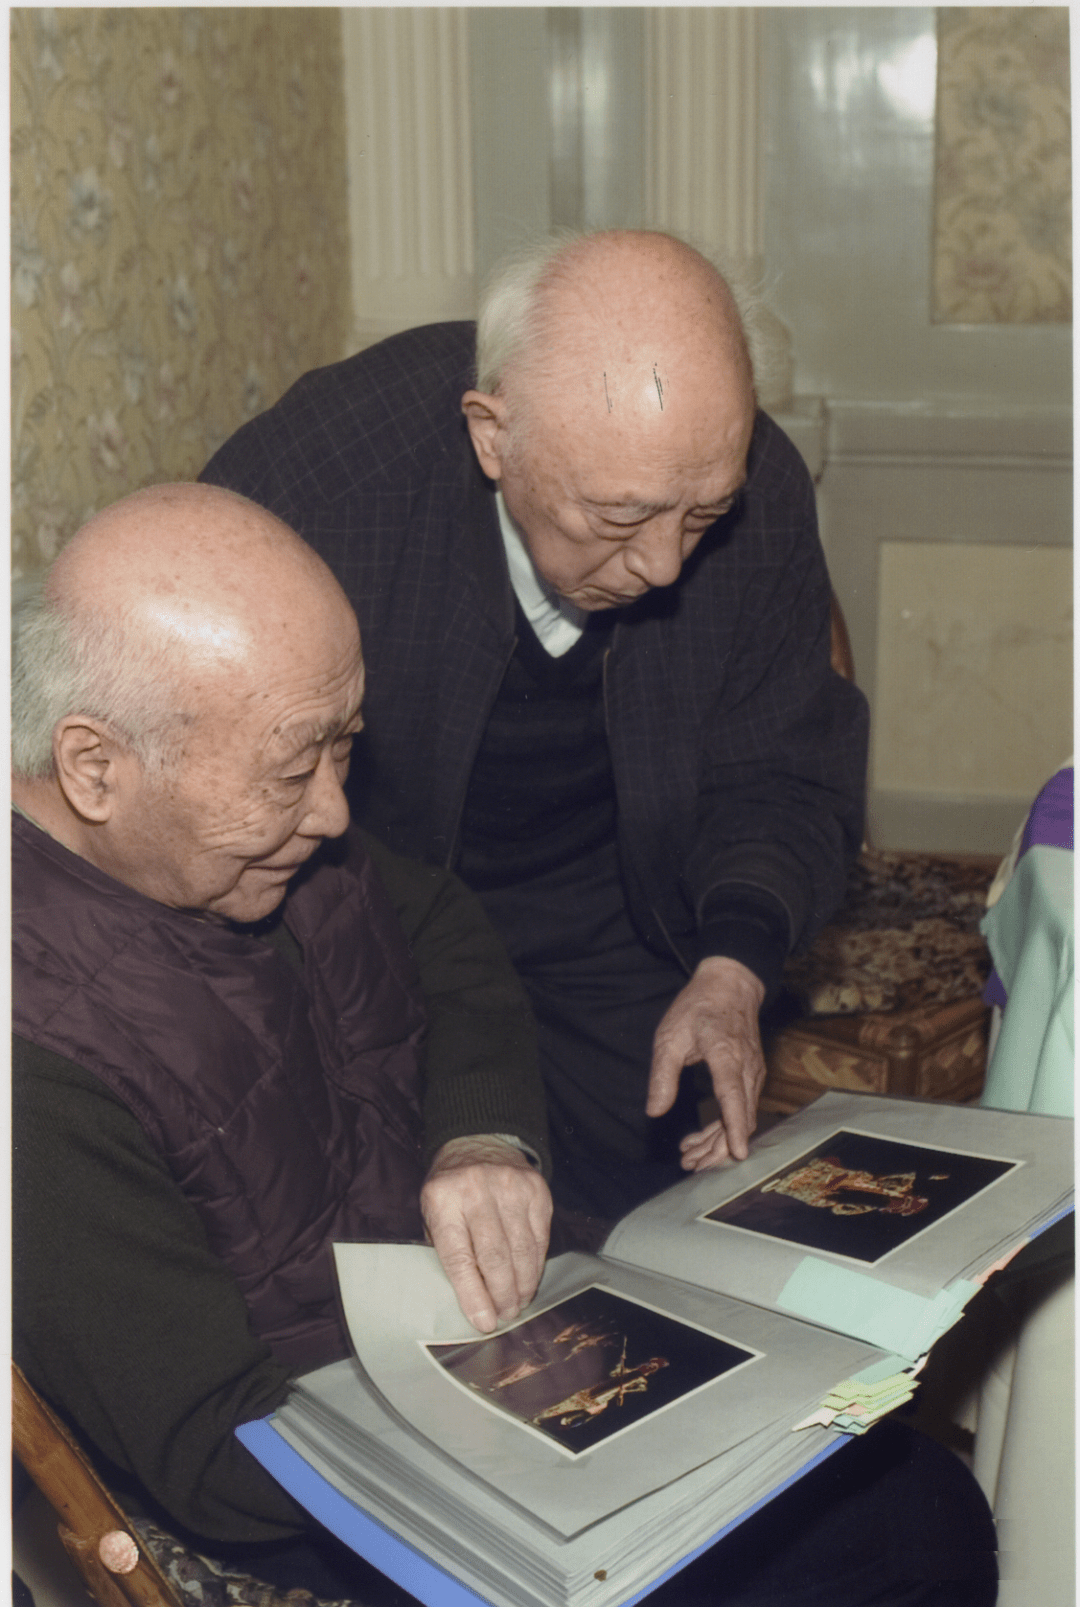
\includegraphics[height=1.38\textwidth,width=1.0\textwidth,viewport=0 0 1050 1550,clip]{Liu-Wu.png}
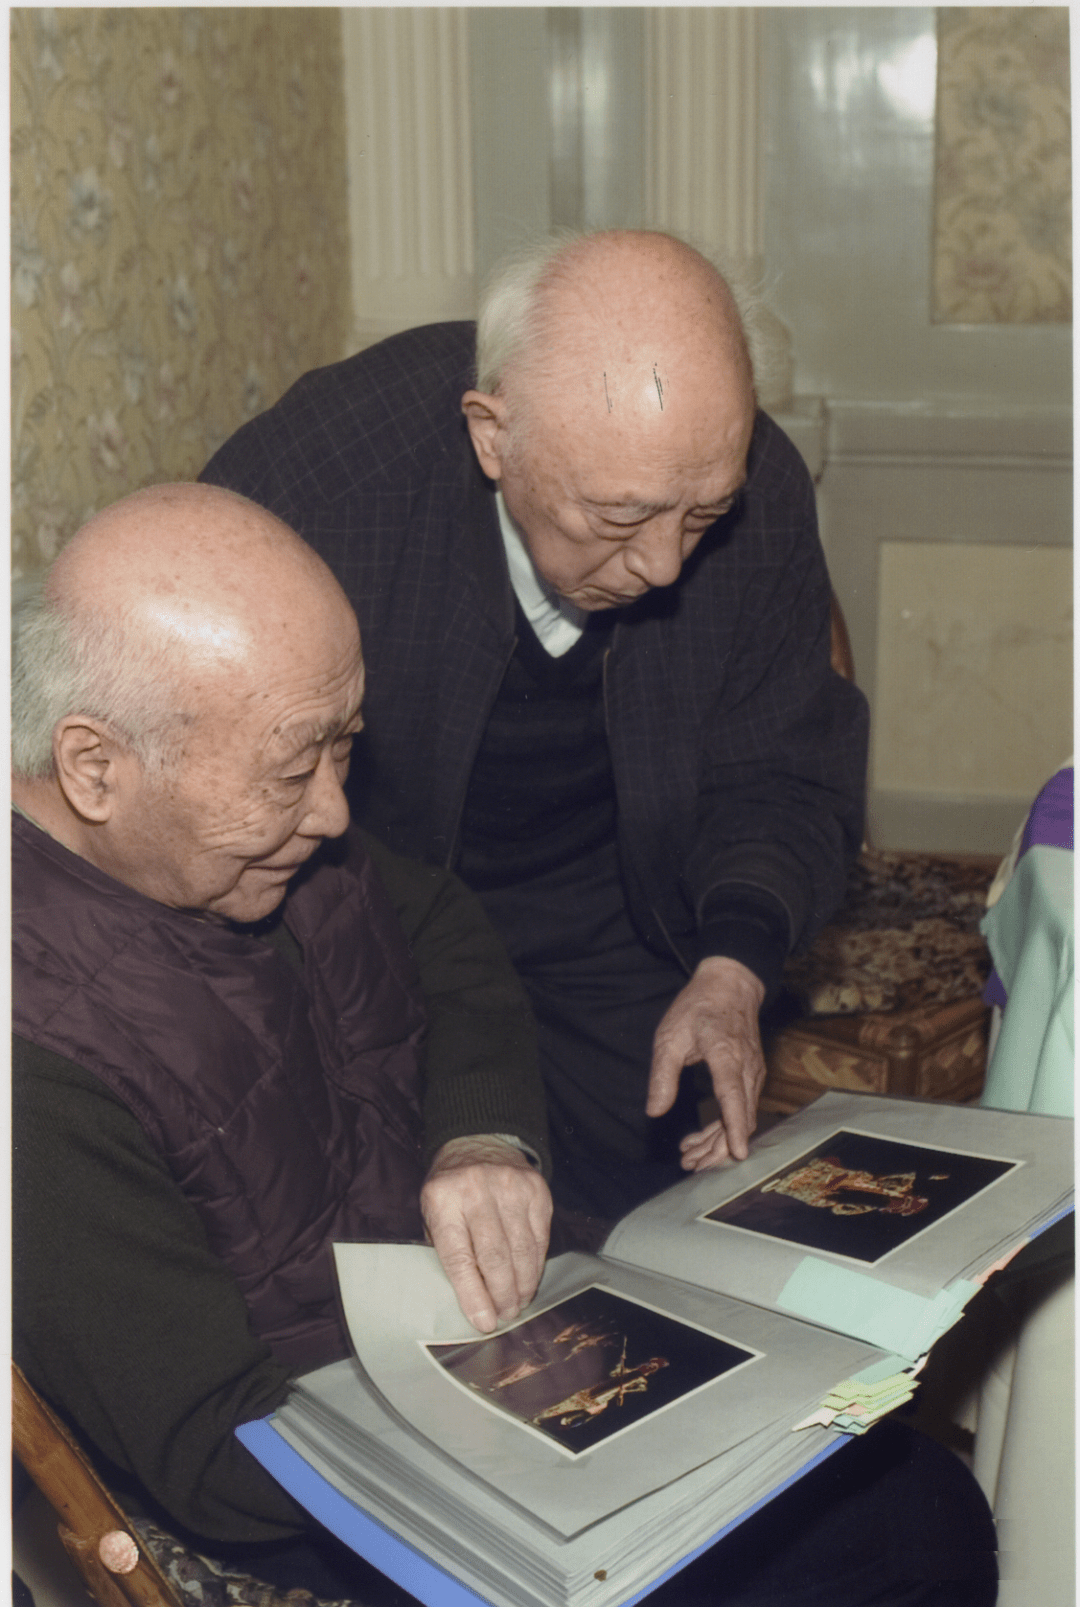
\includegraphics[height=1.38\textwidth,width=1.0\textwidth,viewport=0 0 1050 1550,clip]{Liu-Wu.png}
\caption*{\hei 刘曾复~先生~的主要著作}
\label{Major_Works}
\end{figure}

\newpage
\begin{figure}[h!]
\centering
%\vspace{+0.2in}
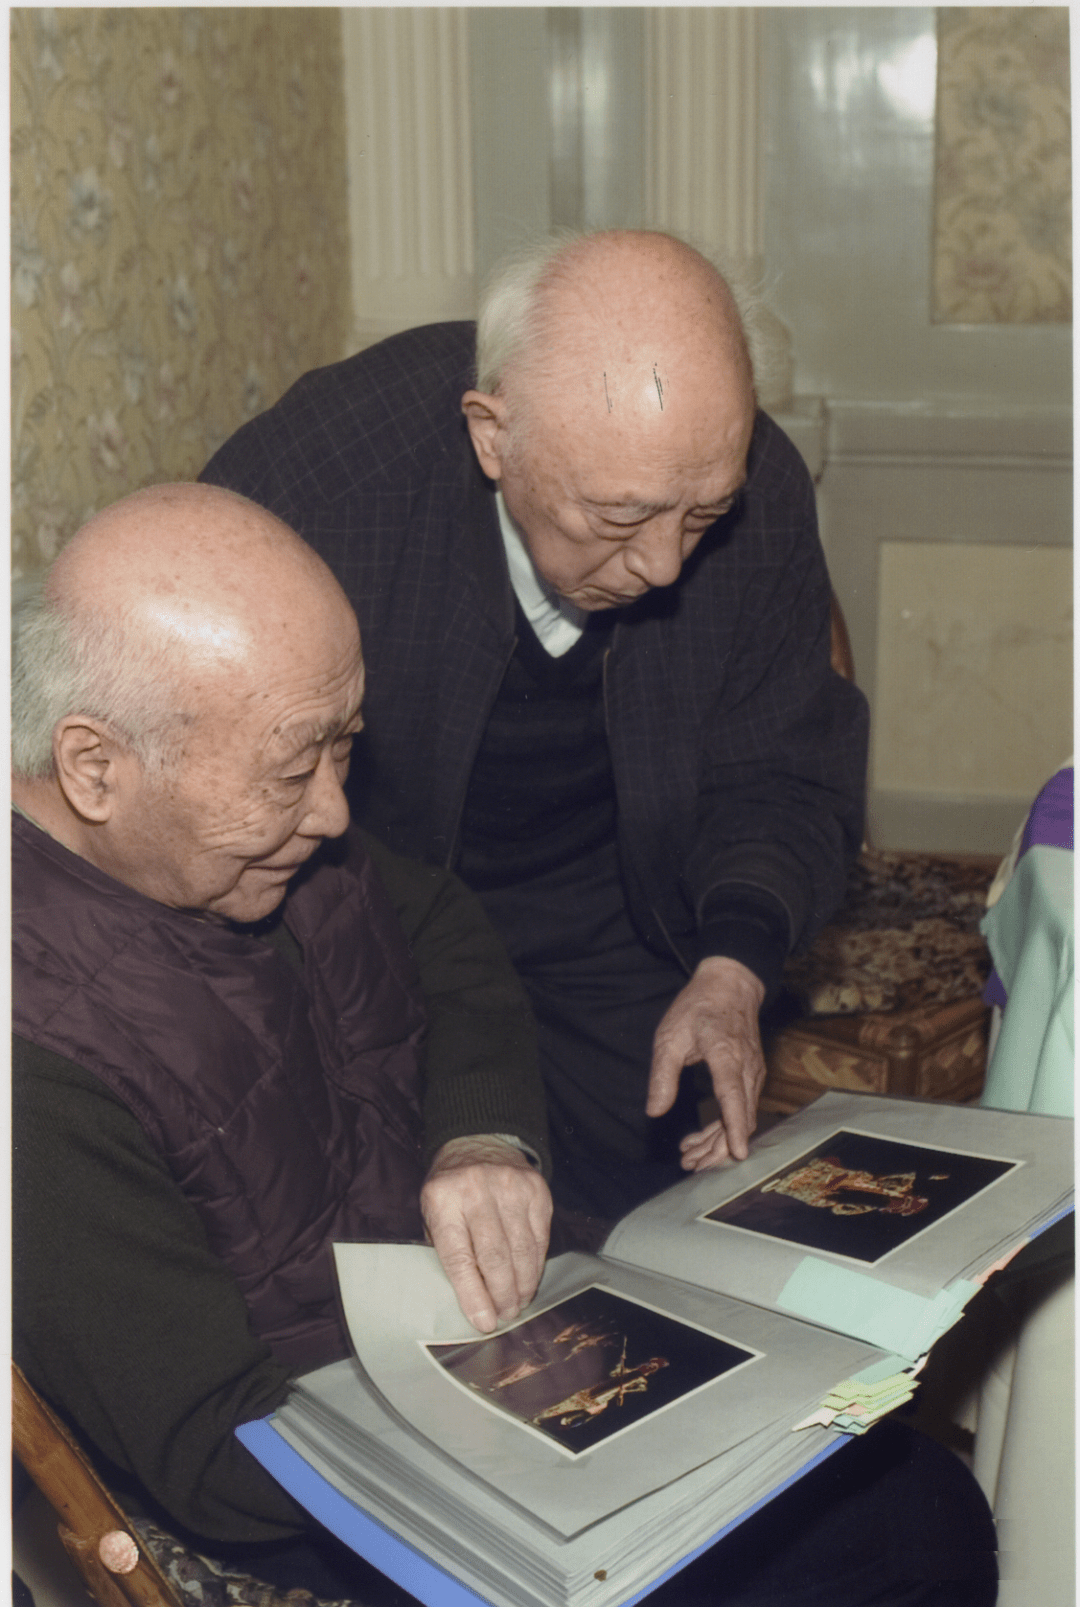
\includegraphics[height=1.38\textwidth,width=1.0\textwidth,viewport=0 0 1050 1550,clip]{Liu-Wu.png}
\caption*{\hei 刘曾复~先生~和~吴小如~先生}
\label{Collect_Liu_Wu}
\end{figure}

\newpage
\begin{figure}[h!]
\centering
%\vspace{-10.5pt}
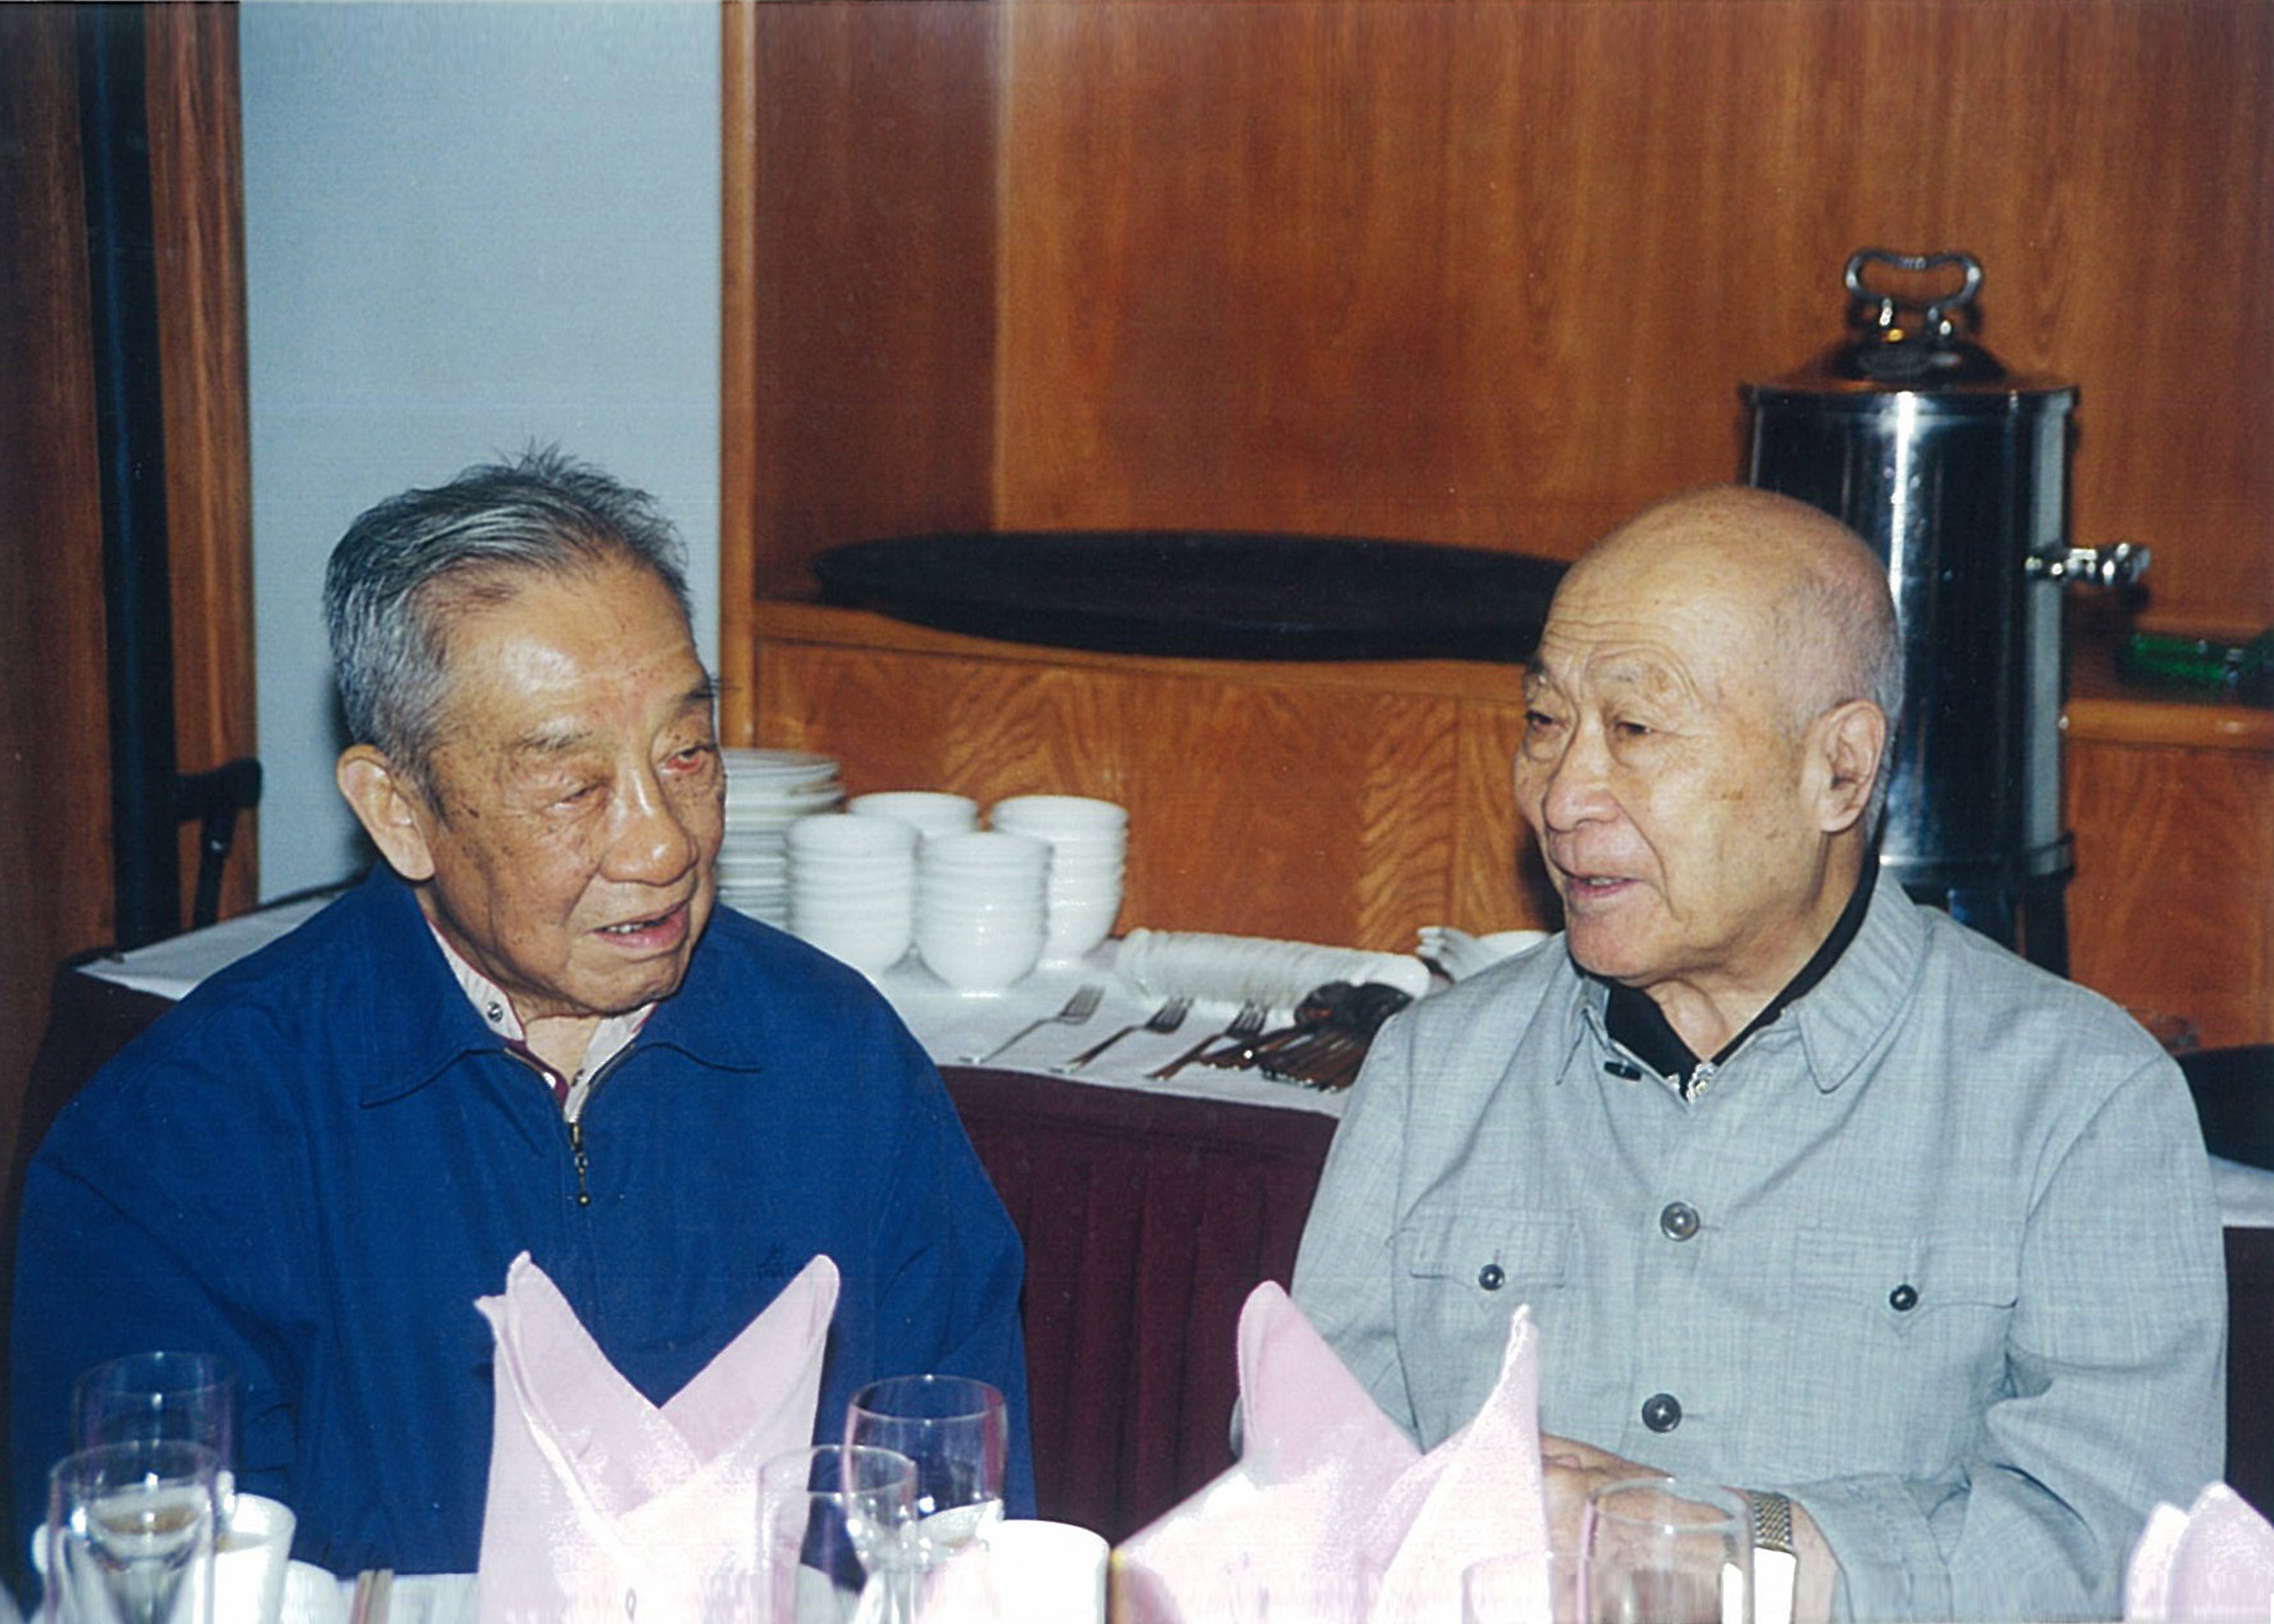
\includegraphics[height=0.60\textwidth,width=1.0\textwidth,viewport=0 0 500 300,clip]{Zhu-Liu.jpg}
\caption*{\hei 朱家溍~先生~和~刘曾复~先生}
\label{Collect_Zhu_Wu}
\end{figure}

\begin{figure}[h!]
\centering
%\vspace{-10.5pt}
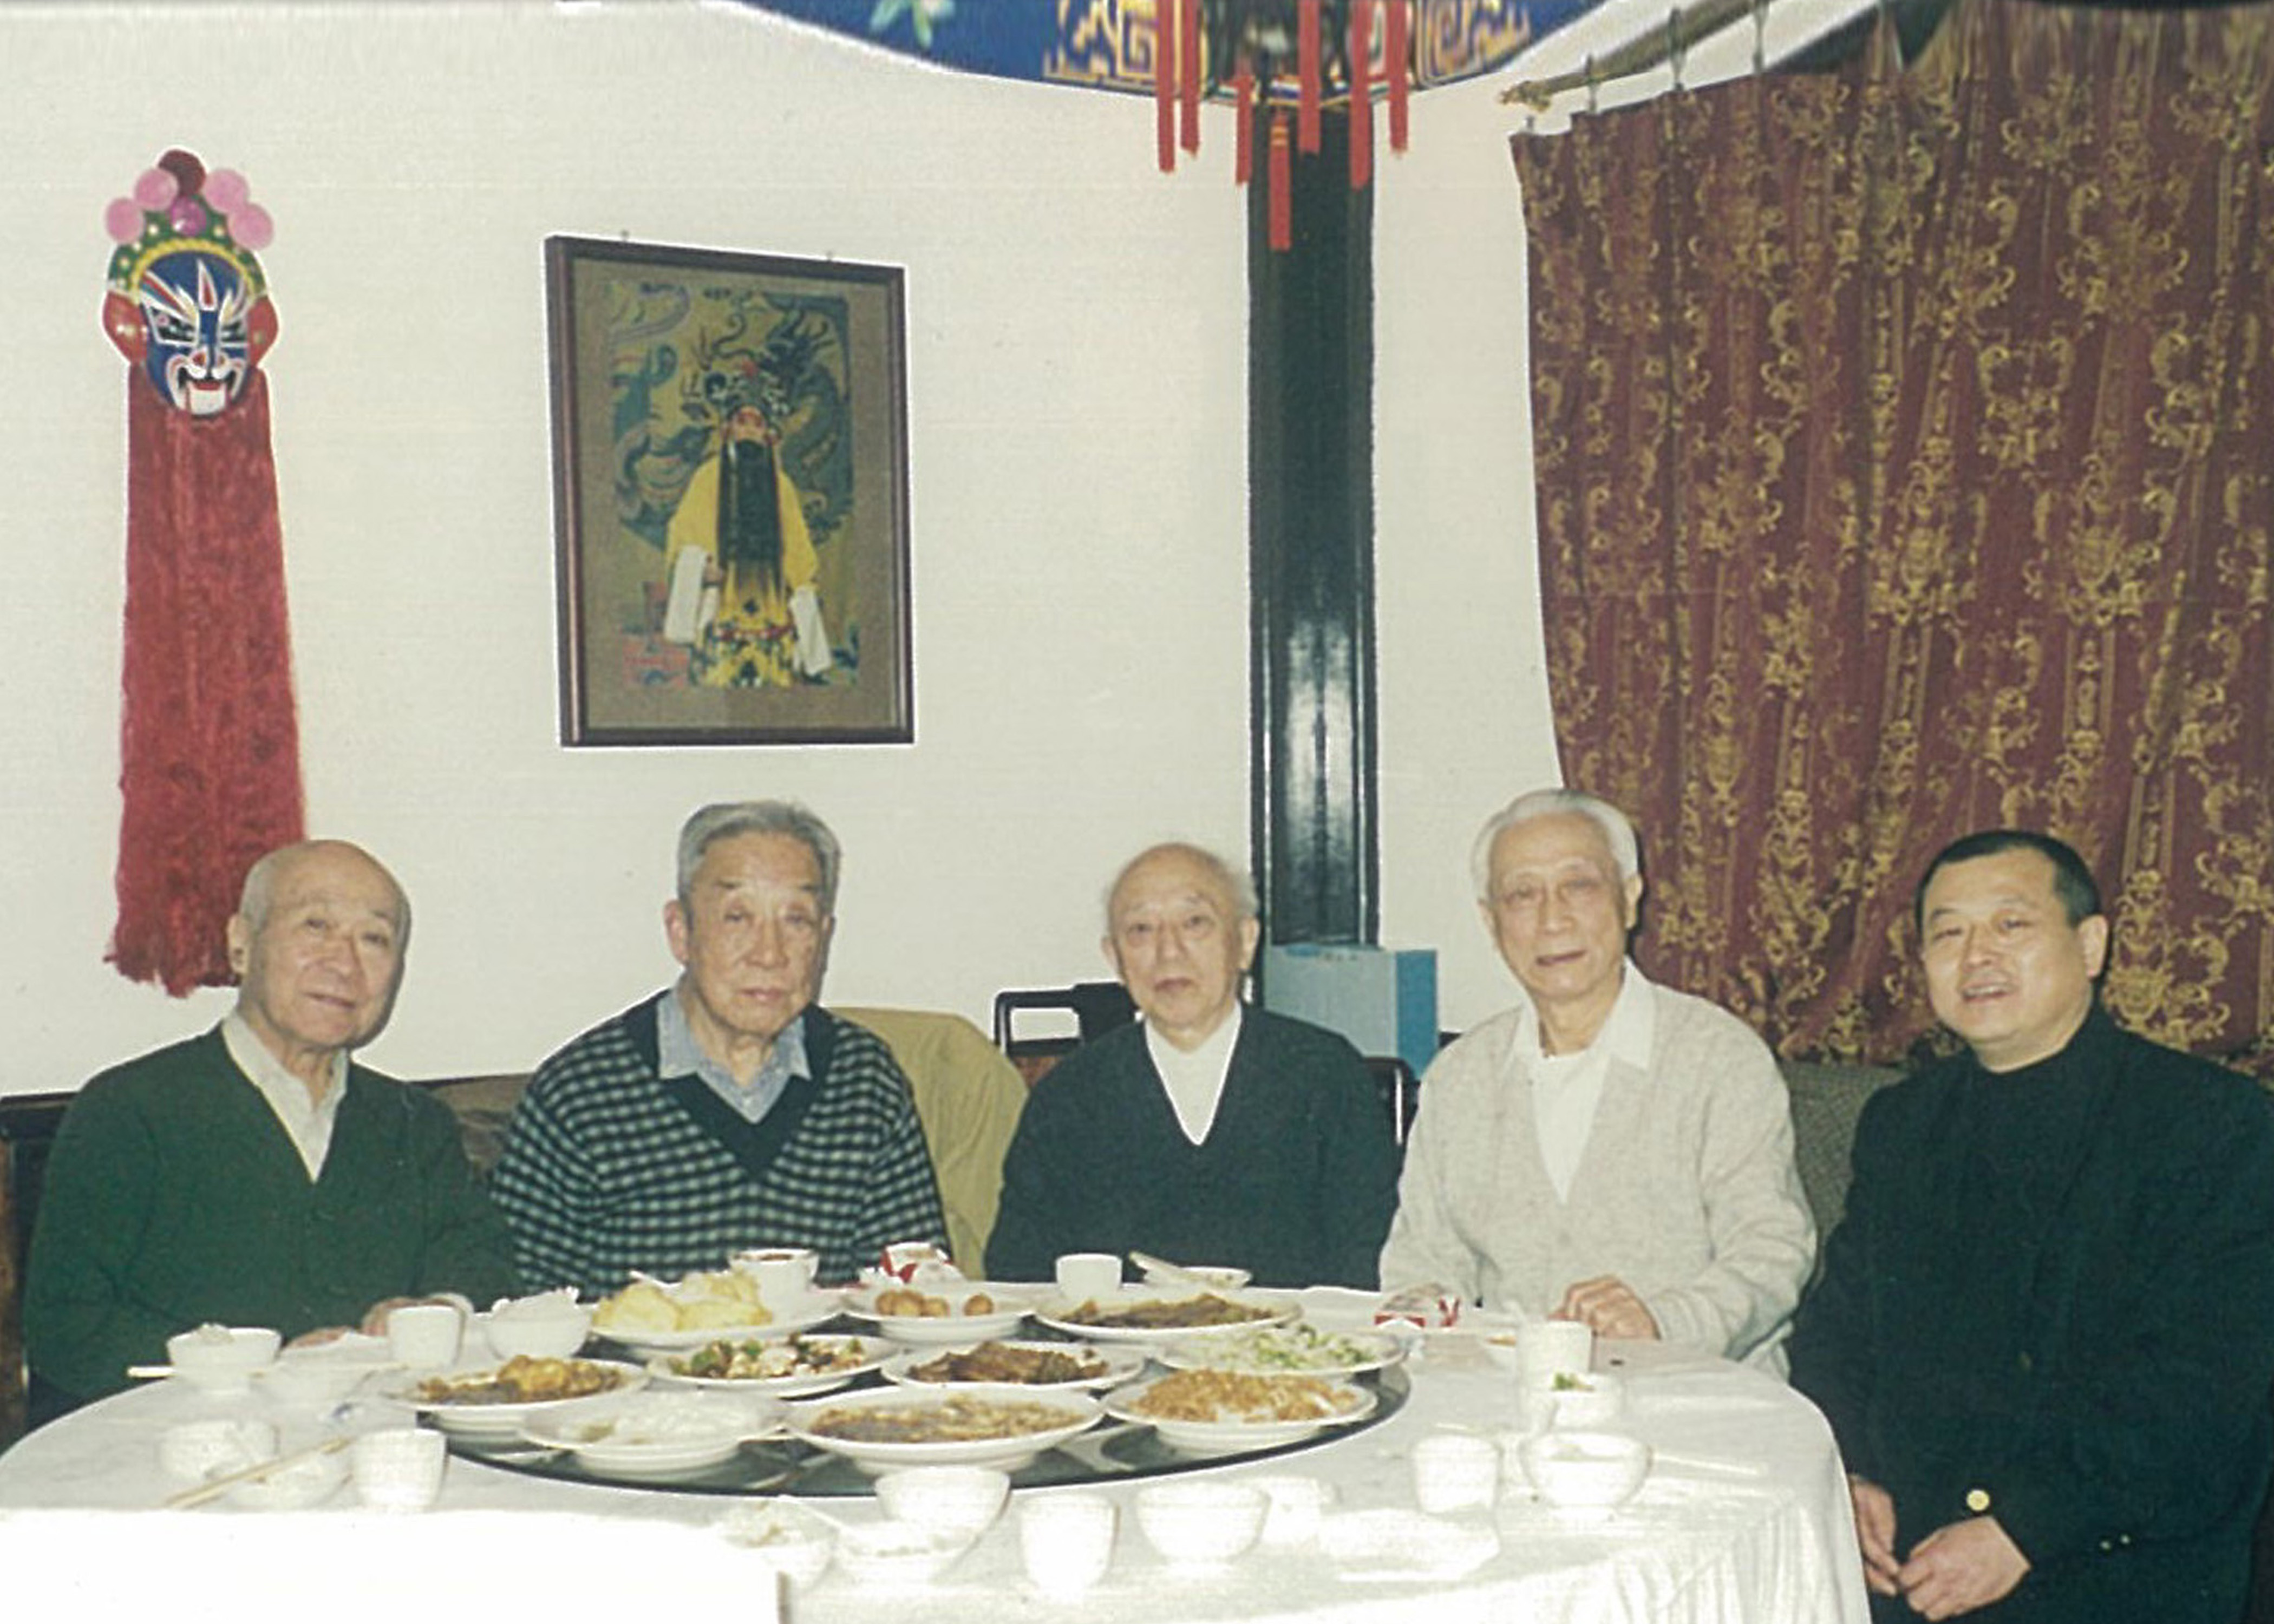
\includegraphics[height=0.60\textwidth,width=1.0\textwidth,viewport=0 0 500 300,clip]{Collect_Zhu-Liu-Wu-Wang.jpg}
\caption*{\hei 左起:~刘曾复~先生、朱家溍~先生、吴小如~先生、王金璐~先生~等~合影}
\label{Collect_Liy_Zhu_Wu_Wang}
\end{figure}
%\keywords{Keyword1; Keyword2; Keyword3}

\newpage
\begin{figure}[h!]
\centering
\vspace{-0.6in}
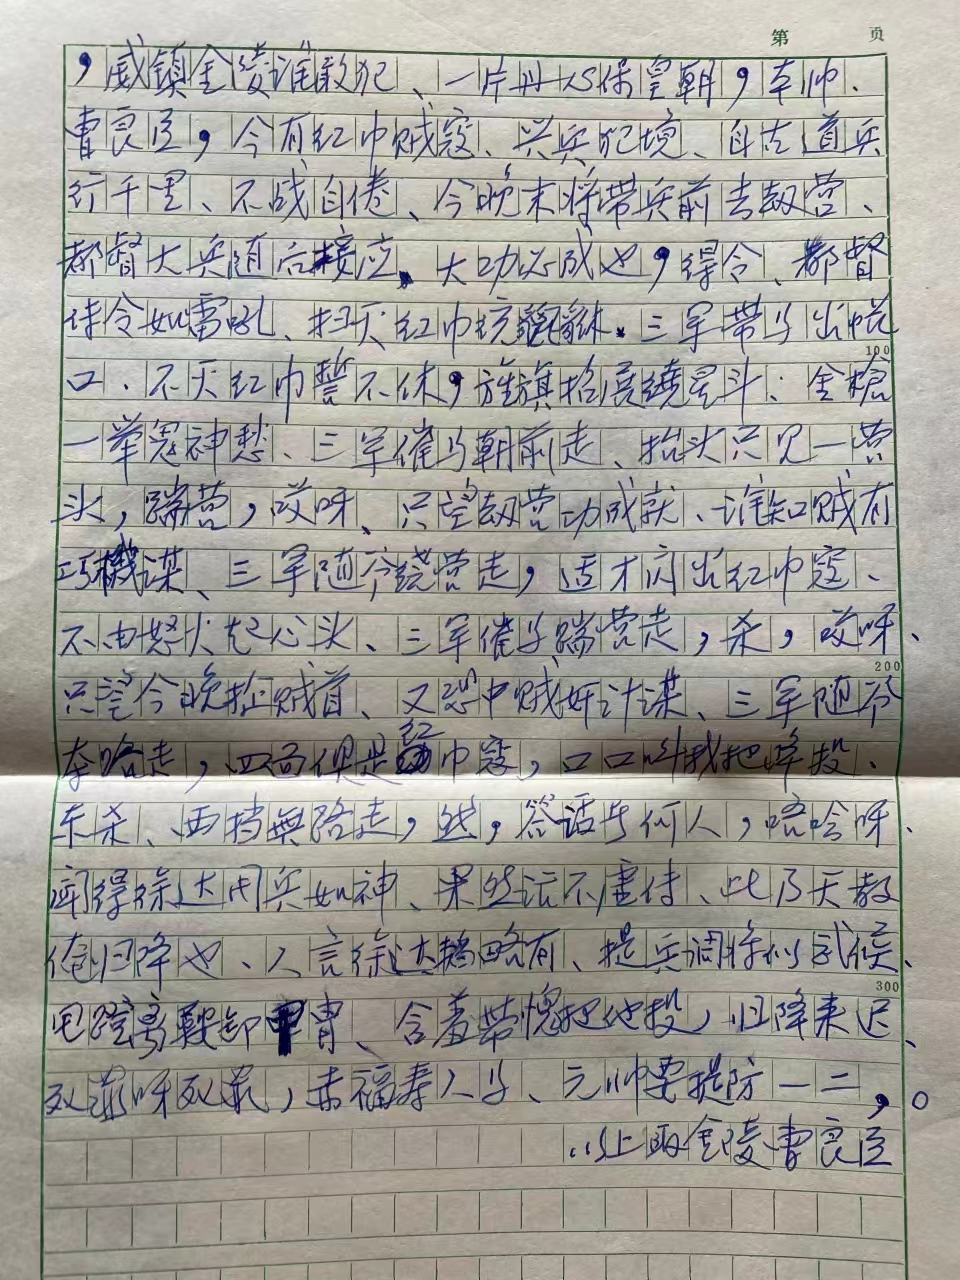
\includegraphics[height=0.68\textwidth,width=0.50\textwidth,viewport=0 0 950 1300,clip]{PekOpe_Liu-1.jpg}
\caption*{\hei 刘曾复~先生~抄录的《取金陵》曹良臣的单词}
\label{Script}
\end{figure}
\vspace{30pt}
\begin{figure}[hbtp!]
\hspace*{-0.5in}
\begin{minipage}[t]{0.53\textwidth}
	\centering
	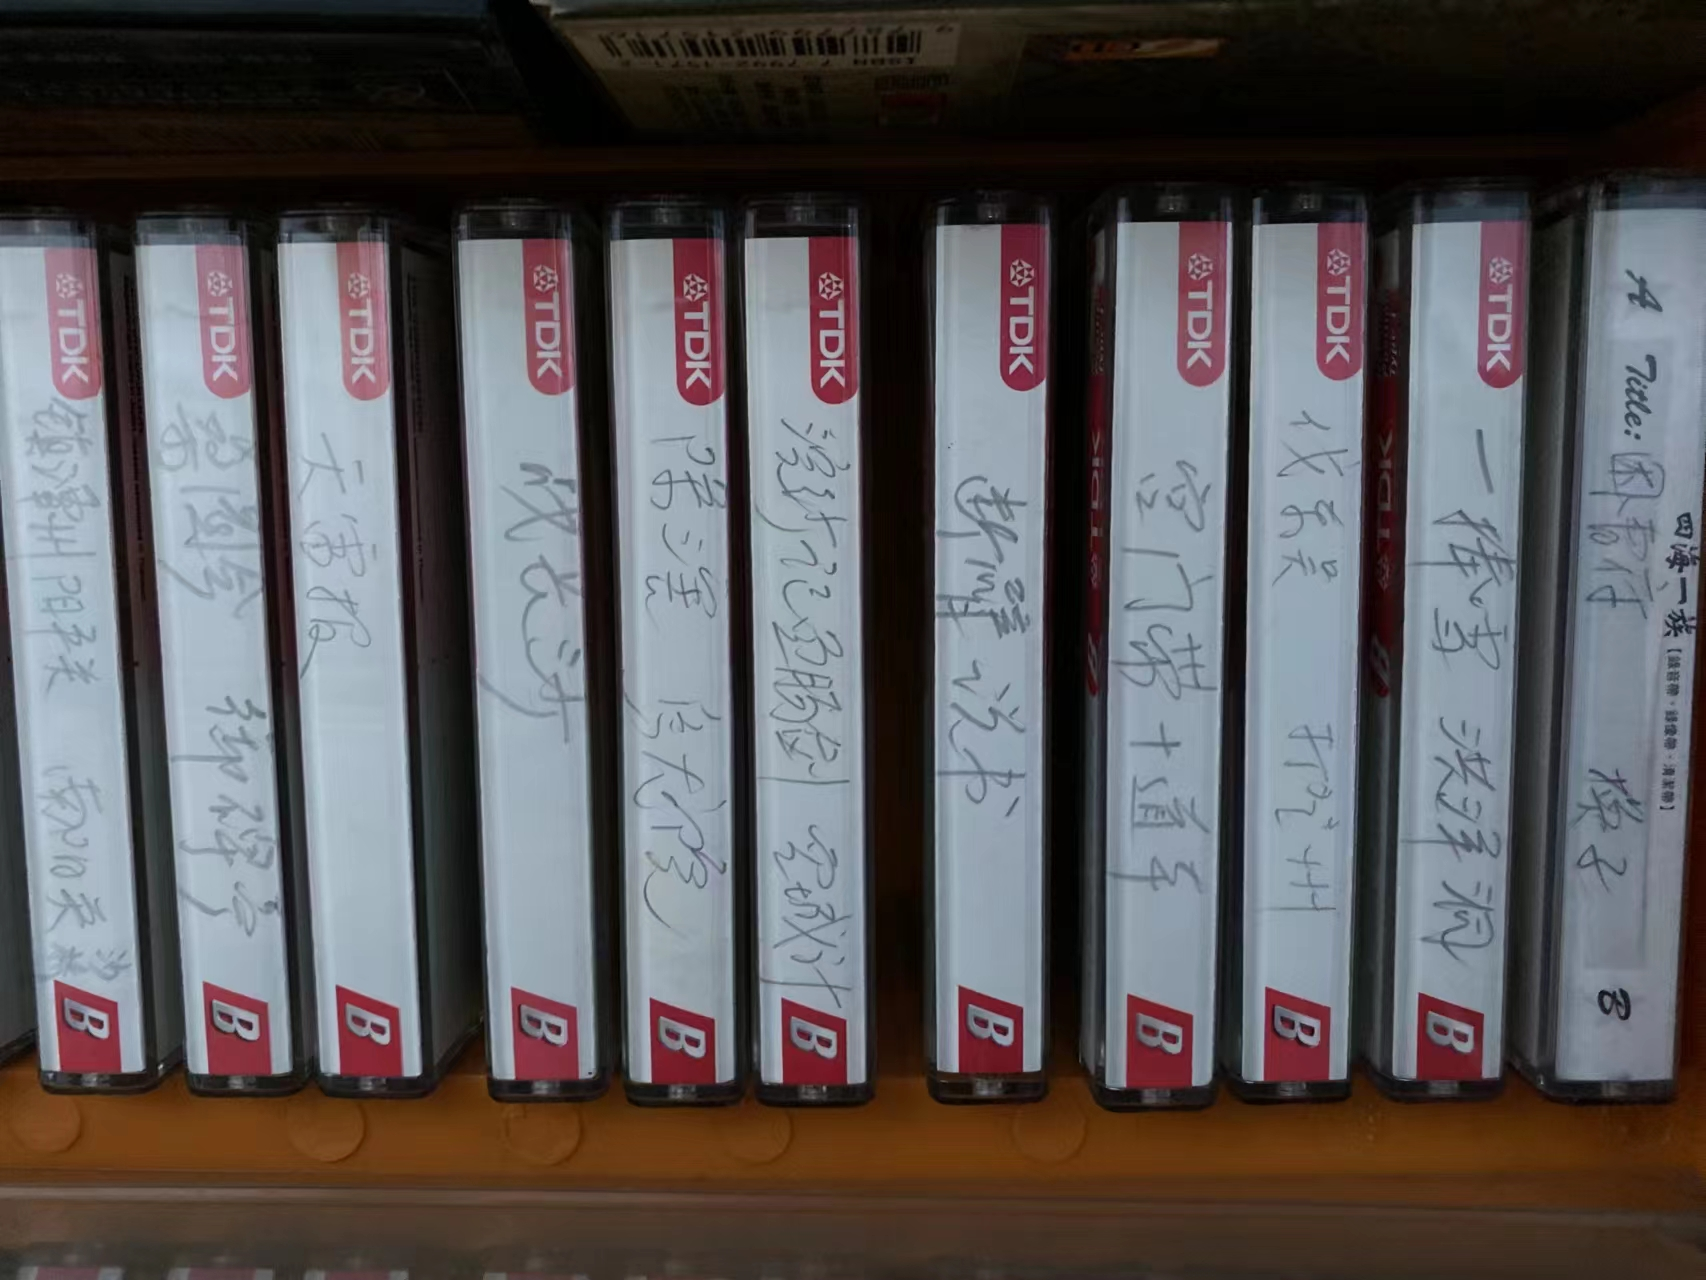
\includegraphics[height=1.00\textwidth,width=1.20\textwidth,viewport=0 0 1750 1300,clip]{PekOpe_Liu-2.jpg}
	\caption*{\hei \fontsize{8.5pt}{4.0pt}\selectfont{左:~刘曾复~先生~保存的部分说戏录音磁带}}
\end{minipage}
\hspace{0.6in}
\begin{minipage}[t]{0.43\textwidth}
	\centering
	\vspace{-3.7in}
	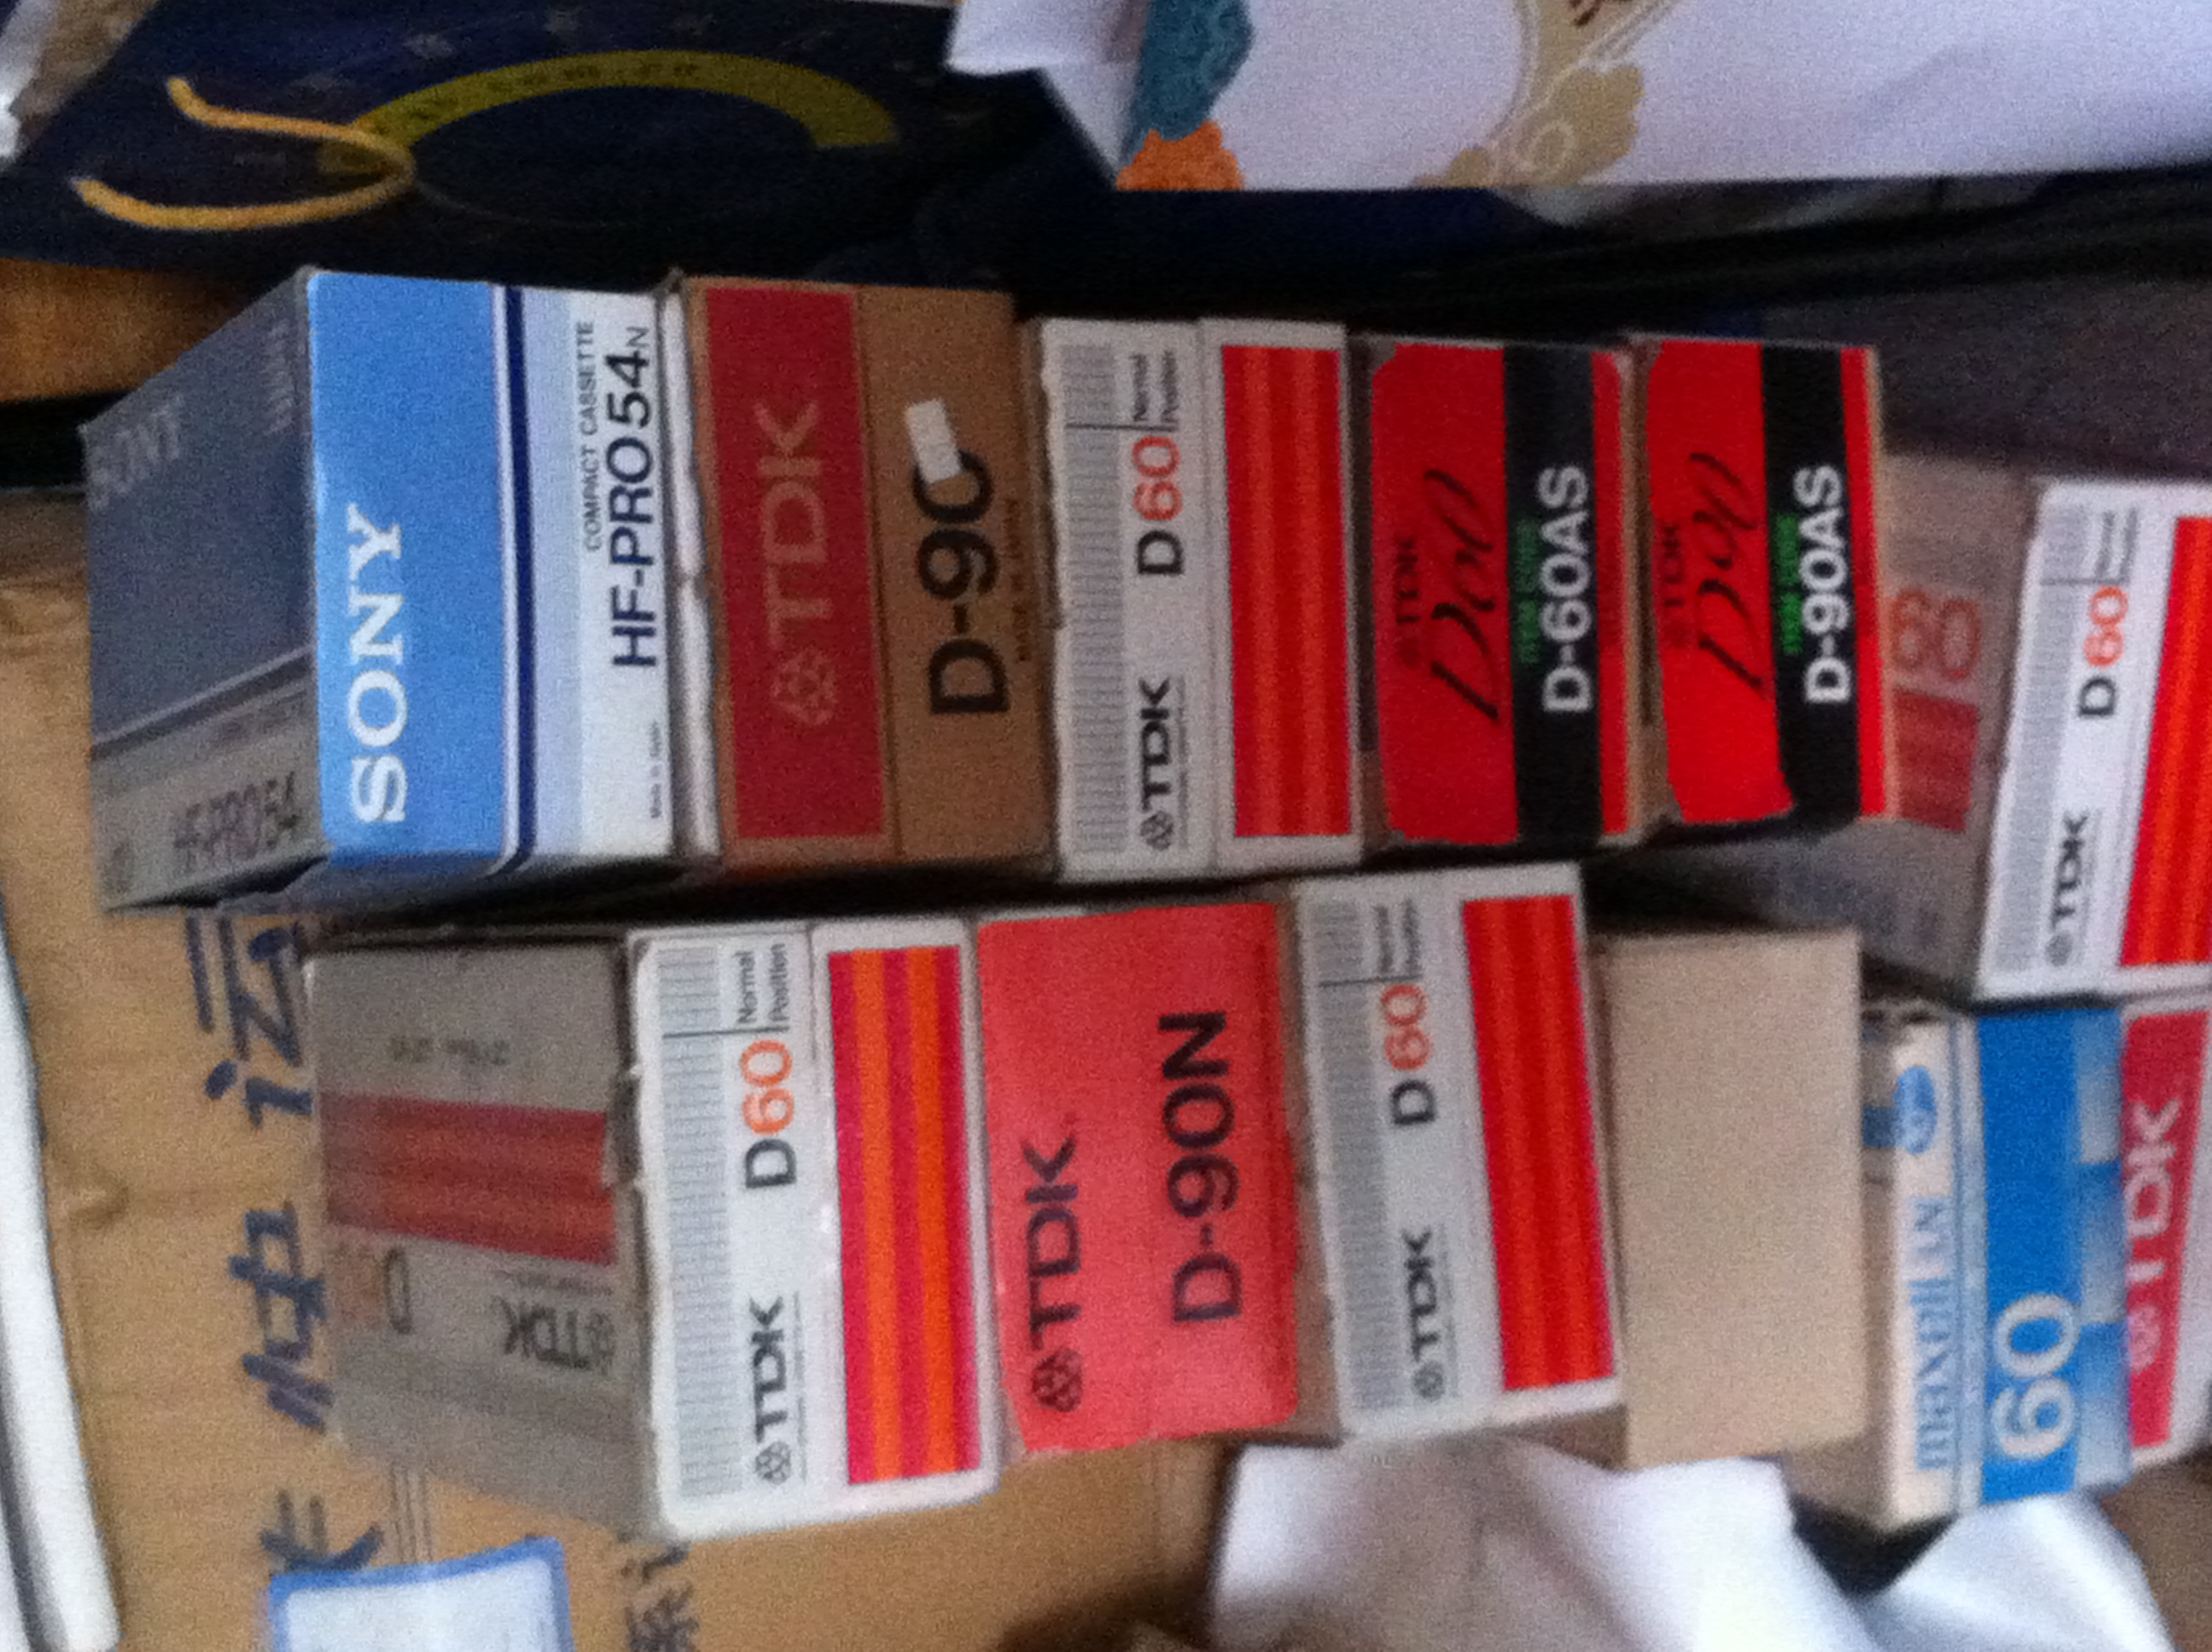
\includegraphics[height=1.10\textwidth,width=1.70\textwidth,angle=270, viewport=0 0 2750 1950,clip]{PekOpe_Wu-5.jpg}
%	\caption*{\hei \fontsize{8.5pt}{4.0pt}\selectfont{右:吴小如~先生~保存的刘曾复先生的说戏录音磁带}}
	\caption*{\hei \fontsize{8.5pt}{4.0pt}\selectfont{右:吴小如~先生~保存的各类说戏录音磁带}}
\end{minipage}
\label{Records}
\end{figure}

